\chapter{Návrh}
Táto kapitola sa venuje návrhu architektúry budúcej aplikácie, s priblížením dvoch hlavných architektúr používaných pri tvorbe webových aplikácií. Následne sú obe porovnané a podľa výsledkov porovnania je vybraná taká, ktorá bude použitá pri vývoji aplikácie. V ďaľšej sekcii sú vymedzené použité technológie budúcou aplikáciou. V neposlednom rade sa kapitola zaoberá návrhom databázy s popisom normalizácie tabuliek a ich zobrazením v schéme v grafickej podobe.

\section{Návrh architektúry}
Dôležitý aspekt pri návrhu aplikácie spočíva vo výbere architektúry, na ktorej bude aplikácia postavená. Na základe jej výberu sa odvíjajú technológie, ktorými bude daná aplikácia disponovať.

V nasledujúcich sekciách sú zdokumentované dva typy architektúr, z ktorých bude na základe porovnania a vlastných skúseností s tvorbou webových aplikácií vybraná jedna, ktorá bude definovať podobu budúcej webovej aplikácie.

\subsection{Architektúra MPA aplikácie}
MPA je skratka pre viac-stránkovú webovú aplikáciu. Takáto aplikácia vždy načíta celú stránku a zobrazí novú v prípade  interakcie s aplikáciou -- zvyčajne po odoslaní formuláru používateľom alebo presmerovaním na inú stránku aplikácie \cite{spa-vs-mpa-1}.

\subsubsection*{Priebeh komunikácie medzi serverom a klientom}
Celkový priebeh komunikácie medzi klientom a serverom zachytáva nasledujúci diagram s jeho popisom.

\begin{figure}[H]
	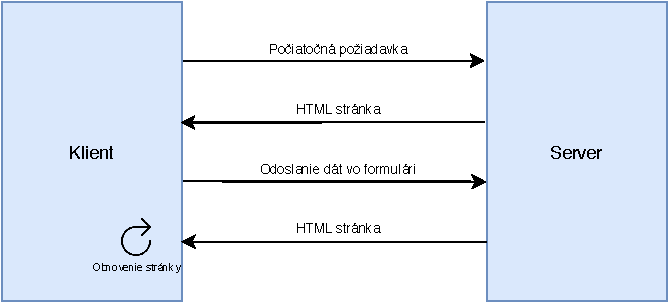
\includegraphics[width=1.0\textwidth]{media/navrh/MPA.pdf}
	\caption{Diagram znázorňujúci architektúru MPA aplikácií}\label{mpa-graf}
\end{figure}

\begin{enumerate}
	\item Klient požiada server o stránku
	\item Server vráti klientovi požadovanú stránku
	\item Klient vrátenú stránku serverom vykreslí
	\item Klient vyplní formulár, ktorý sa následne odošle na server
	\item Server prijme údaje od klienta, ktoré následne spracuje
	\item Po spracovaní údajov klientovi vráti späť stránku s aktualizovanými údajmi
	\item Klient túto stránku načíta, čím príde k obnoveniu stránky
\end{enumerate}

Technológia AJAX čiastočne rieši problém znovunačítavania celej stránky dynamickým aktualizovaním tých častí aplikácie, ktoré boli používateľom zmenené. Avšak zakomponovanie tejto technológie do MPA sťažuje a komplikuje celý vývojový proces aplikácie \cite{mpa-architektura}.

\subsubsection*{Výhody použitia MPA architektúry}

\begin{itemize}
	\item Jednoduchá optimalizácia stránok pre webové vyhľadávače \cite{spa-vs-mpa-1}
	\item Umožňuje jednoduchú správu informácií na jednotlivých stránkach \cite{spa-vs-mpa-3}
	\item Je potrebný menší rozsah nástrojov a znalostí narozdiel od vývoja SPA aplikácie \cite{spa-vs-mpa-2}
	\item Veľa dostupných riešení pre vývoj MPA aplikácií \cite{spa-vs-mpa-2}
\end{itemize}


\subsubsection*{Nevýhody použitia MPA architektúry}

\begin{itemize}
	\item Zvýšený čas načítavania stránok kvôli neustálemu obnovovaniu stránok (neplatí pri použití technológie AJAX) \cite{spa-vs-mpa-1}
	\item Znížený výkon aplikácie, kvôli neustálemu načítavaniu väčšieho množstva informácií naraz pred následným poslaním stránky používateľovi \cite{spa-vs-mpa-1}
	\item Úzka previazanosť vývoja aplikácie na strane servera a klienta, čo znemožňuje prípadné neskoršie nasadenie rôznych technológií \cite{spa-vs-mpa-2}
\end{itemize}


\subsection{Architektúra SPA aplikácie}
SPA je skratka pre single-page aplikáciu. Single-page aplikácia je aplikácia, ktorá nepotrebuje znovunačítanie stránky počas jej používania. Na tomto type architektúry sú postavené aplikácie ako Gmail\footnote{https://gmail.com}, Google Mapy\footnote{https://maps.google.com}, Facebook\footnote{https://facebook.com} či GitHub\footnote{https://github.com}. V tomto prípade sa o aktualizáciu obsahu na stránke nestará server, ale klient, zväčša pomocou frameworku\footnote{Sada podporných programov uľahčujúca vývoj aplikácie} bežiacom v prostredí webového prehliadača \cite{spa-vs-mpa-3}.

\subsubsection*{Priebeh komunikácie medzi serverom a klientom}
Celkový priebeh komunikácie medzi klientom a serverom zachytáva nasledujúci diagram s jeho popisom.

\begin{figure}[H]
	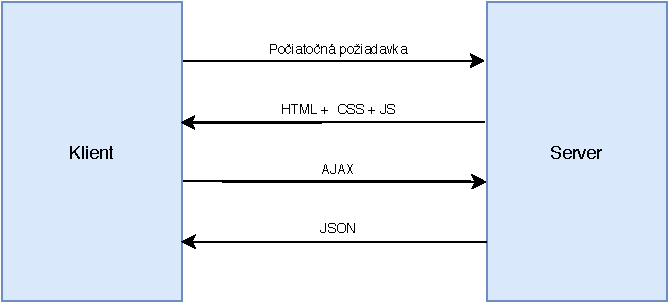
\includegraphics[width=1.0\textwidth]{media/navrh/SPA.pdf}
	\caption{Diagram znázorňujúci architektúru SPA aplikácií}\label{spa-graf}
\end{figure}

\begin{enumerate}
	\item Klient požiada server o stránku
	\item Server vráti klientovi požadovanú HTML stránku so všetkým obsahom aplikácie
	\item Klient vrátenú stránku serverom vykreslí
	\item Klient vyplní formulár, ktorý sa následne odošle na server pomocou AJAXu
	\item Server prijme údaje od klienta, ktoré následne spracuje
	\item Po spracovaní údajov server vráti späť klientovi aktualizované údaje (v JSON\footnote{Formát na výmenu dát medzi klientom a serverom \cite{co-je-json} } formáte)
	\item Klient zahodí staré údaje na stránke a nahradí ich novými, čím príde k obnoveniu údajov ale nie stránky
\end{enumerate}


\subsubsection*{Výhody použitia SPA architektúry}

\begin{itemize}
	\item Rýchlosť a responzívnosť aplikácie založenej na aktualizovaní iba tej časti aplikácie, ktorá sa zmenila \cite{spa-vs-mpa-1}
	\item Minimálna previazanosť kódu aplikácie na strane servera a klienta, čo umožňuje jednoduchú správu používaných knižníc bez ovplyvnenia ďalších častí aplikácie \cite{spa-vs-mpa-2}
	\item Zjednodušení proces vývoja, nakoľko sa o vykreslenie obsahu nestará server ale klientský framework \cite{spa-vs-mpa-3}
\end{itemize}


\subsubsection*{Nevýhody použitia SPA architektúry}

\begin{itemize}
	\item Ťažká optimalizácia aplikácie pre webové vyhľadávače, nakoľko sa o vykreslenie obsahu stará Javascript\footnote{Programovací jazyk bežiaci vo webovom prehliadači}, ktorý webové vyhľadávače neinterpretujú \cite{spa-vs-mpa-1}
	\item Prvé načítanie aplikácie trvá dlhší čas v porovnaní s MPA architektúrou, pretože sa musí všetok obsah aplikácie stiahnuť do zariadenia
	\item Nemožnosť zobrazenia aplikácie pri vypnutom Javascripte vo webovom prehliadači \cite{spa-vs-mpa-2}
\end{itemize}


\subsection{Voľba architektúry}

Pre budúcu aplikáciu som sa rozhodol vybrať SPA architektúru, nie len z dôvodu rýchlejšieho a jednoduchšieho procesu vývoja, ale aj vďaka vlastným skúsenostiam z oblasti vývoja SPA aplikácií. Nakoľko aplikácia bude dostupná iba vopred vybraním používateľom, nebude potrebné ju optimalizovať pre webové vyhľadávače.

\section{Voľba technológií}
V tejto sekcii sa presunieme od voľby architektúry, na ktorej bude aplikácia postavená, ku voľbe technológií, ktoré budu použité vo výslednej aplikácii.

\subsection{PHP}
Medzi zvolené technológie bude jednoznačne patriť programovací jazyk PHP, nakoľko jeho voľba je jedným z nefunkčných požiadaviek kladených na budúcu aplikáciu. 

\subsubsection*{Framework}
Vývoj softvéru je komplexný proces, ktorý zahŕňa nie len výslednú implementáciu konkrétneho softvéru, ale aj analýzu, návrh, a v neposlednom rade aj testovanie softvéru. Softvérové frameworky uľahčujú prácu vývojárom tým, že im umožňujú prevziať kontrolu nad celým procesom vývoja softvéru alebo jeho väčšiny \cite{co-je-framework}.

Medzi niektoré výhody použitia frameworku patrí:

\begin{itemize}
	\item Pomoc pri zavádzaní lepších programovacích postupov a vhodnom využívaní návrhových vzorov
	\item Väčšia bezpečnosť výsledného kódu
	\item Možnosť vyhnúť sa duplicite kódu
	\item Skrátenie času vývoju výslednej aplikácie
\end{itemize}

Pre vývoj webových aplikácií v PHP existujú viaceré frameworky, ako napríklad CakePHP\footnote{https://cakephp.org}, Nette\footnote{https://nette.org}, Symfony\footnote{https://symfony.com}, Laravel\footnote{https://laravel.com} a iné.
Spomedzi menovaných bol vybraný na základe skúseností posledný z nich -- Laravel.

\subsection{HTML 5}
HTML -- HyperText Markup Language -- je značkovací jazyk používaný pre definovanie významu a štruktúry dokumentov. Ako už z názvu vyplýva, HTML používa značky pre definovanie elementov v dokumente s rozdielnymi vlastnosťami, ako napríklad nadpis, odstavec, tabuľky a iné.
Tieto značky sú interpretované webovým prehliadačom, ktorý ich následne vykreslí na stránku \cite{co-je-html}.

Najnovšou verziou tohto jazyka je verzia HTML 5.

\subsection{CSS 3}
Cascading Style Sheets (CSS) je jazyk, ktorý sa používa na ilustráciu vzhľadu, štýlu a formátu dokumentu a jeho elementov napísaného v akomkoľvek značkovacom jazyku. Využíva sa najmä v spojitosti s webovými stránkami. CSS je tvorený pravidlami aplikovanými na jednotlivé elementy dokumentu. Tieto pravidlá sú definované selektorom elementu, ktorý určuje polohu elementu v dokumente, a CSS pravidlami rôzneho typu, ktoré definujú konkrétny štýl daného elementu \cite{co-je-css}. 

CSS3 je momentálne najnovšia verzia jazyka CSS.

\subsection{JavaScript}
JavaScript je jednoduchý programovací jazyk, pomocou ktorého môžu vývojári webových stránok vytvárať interaktívne a dynamické webové stránky. Bol vyvinutý spoločnosťou Netscape, ale v súčasnosti ho používa väčšina webových prehliadačov. Je to programovací jazyk s otvoreným zdrojovým kódom, ktorý môže ktokoľvek používať \cite{co-je-js}.

\subsubsection*{Framework}
Nakoľko novnovznikajúca aplikácia bude postavená na SPA architektúre, bude potrebné, aby sa stránky vykresľovali na strane klienta. To sa dá samozrejme dosiahnuť bez použitia frameworku, ktorý by sa postaral o aktualizáciu komponentov na stránke, avšak z dôvodu rýchlejšieho procesu vývoja som sa rozhodol použiť framework Vue.js\footnote{https://vuejs.org}.

Vue.js je progresívny framework pre vytváranie používateľských rozhraní. Tento framework bol navrhnutý od základov tak, aby bol postupne prispôsobiteľný. Nakoľko je zameraný iba na vrstvu zobrazenia, je ľahké ho integrovať s inými knižnicami a existujúcimi projektmi \cite{co-je-vue}.

Pre vytváranie používateľského rozhrania existujú aj iné frameworky, ako napríklad React\footnote{https://reactjs.org} a Angular\footnote{https://angular.io}, avšak z dôvodu doterajších skúseností autora bol zvolený Vue.js framework.

\section{Návrh databázy}
V predchádzajúcej kapitole v podsekcii \ref{sucasny-model-db} bol zanalyzovaný databázový model súčasnej aplikácie.

Táto sekcia popíše normalizáciu súčasnej databázy a na základe poznatkov vyplývajúcich z analýzy o súčasnom databázovom modeli bude navrhnutý databázový model pre vznikajúcu aplikáciu, ktorý bude brať do úvahy funkčné požiadavky kladené na aplikáciu.

\subsection{Normalizácia databázy}
Normalizácia databázy je proces efektívneho usporiadania údajov v databáze. Tento proces má dva ciele: odstránenie nadbytočných údajov (napríklad neukladanie tých istých údajov vo viac ako jednej tabuľke) a zabezpečenie ukladania iba  súvisiacich údajov do tabuľky. Normalizovaná databáza znižuje množstvo miesta potrebného na ukladanie dát a navyše zabezpečí, že dáta sú logicky usporiadané \cite{co-je-normalizacia}.

Pri návrhu databázy je žiaduce dosiahnuť tretiu normálovú formu (3NF) pre každú tabuľku v databáze, pretože až takáto databáza sa považuje za normalizovanú \cite{normalizovana-tabulka}.

Proces normalizácie tabuľky zahŕňa jej konverziu do prvej normálovej formy (ak v nej nie je), následne do druhej normálovej formy (ak ju nespĺňa) a na koniec do tretej normálovej formy.

Tabuľka je v prvej normálovej forme (1NF), ak spĺňa nasledujúce vlastnosti \cite{typy-normalizacie}:
\begin{itemize}
	\item obsahuje iba atomické hodnoty v každom stĺpci
	\item hodnoty uložené v stĺpci sa viažu iba na daný stĺpec
	\item všetky stĺpce v tabuľke majú unikátny názov
	\item nezáleží na poradí ukladania dát do stĺpcov 
\end{itemize}

Tabuľka je v druhej normálovej forme (2NF), ak má nasledujúce vlastnosti \cite{typy-normalizacie}:
\begin{itemize}
	\item tabuľka spĺňa 1NF
	\item nemôže obsahovať čiastočnú závislosť
\end{itemize}

Čiastočná závislosť v tabuľke existuje pokiaľ atribút v tabuľke závisí od časti primárneho kľúča a nie od celého kľúča \cite{ciastocna-zavislost}. 

Na to aby tabuľka bola v tretej normálovej forme (3NF), musí navyše mať nasledujúce vlastnosti \cite{typy-normalizacie}:
\begin{itemize}
	\item tabuľka spĺňa 2NF
	\item nemôže obsahovať tranzitívnu závislosť
\end{itemize}

Tranzitívna závislosť predstavuje tri alebo viac atribútov, ktoré majú funkčnú závislosť medzi sebou, čo znamená, že stĺpec A závisí na stĺpci B cez stĺpec C \cite{tranzitivna-zavislost}.

\subsubsection*{Tabuľka czkp\_vrh}
Na základe analýzy a splnenia požiadavky 3NF bude potrebné, aby údaje o chovateľovi sa nenachádzali priamo v tabuľke vrhov, ale cez cudzí kľúč smerujúci do tabuľky určenej pre chovateľov/majiteľov.
Taktiež bude potrebné presunúť údaje o registrácii vrhu a poznámok do tabuliek pre ne určených.

\subsubsection*{Tabuľka czkp\_zvire}
Z vykonanej analýzy tejto tabuľky vyplýva, že tabuľka okrem údajov o samotnom zvierati obsahuje navyše informácie o entitách ako majiteľ/chovateľ, registrácia zvieraťa, prípadne poznámky viažuce sa k danému zvieraťu. Pretože výsledná tabuľka má byť normalizovaná, nemala by obsahovať tieto údaje priamo, ale cez cudzí kľúč.

Pre každú horeuvedenú entitu by mala vzniknúť jedna tabuľka --- zvlášť pre chovateľov a majiteľov, registrácie zvierat a poznámky. Z pohľadu databázy netreba rozoznávať ľudí, či sú daní ľudia chovateľmi alebo majiteľmi, preto môžu byť uložení v jednej tabuľke.

\subsubsection*{Tabuľka czkp\_mimi}
Analýza tejto tabuľky ukázala, že by tabuľka spĺňala 3NF v prípade, ak by stĺpec chovateľa obsahoval cudzí kľúč namiesto textu.
Pri porovnaní tejto tabuľky a tabuľky \mintinline{php}{czkp_zvire} je možné vidieť, že stĺpce definované v tejto tabuľke sa štruktúrou rovnajú stĺpcom v tabuľke \mintinline{php}{czkp_zvire}, z čoho vyplýva, že táto tabuľka môže byť spojená s tabuľkou \mintinline{php}{czkp_zvire}.

\subsubsection*{Tabuľka pp\_informace}
Táto tabuľka je obdobou tabuľky \mintinline{php}{czkp_vrh}, čo znamená, že tieto dve tabuľky môžu byť zlúčené do jednej, po oddelení údajov o registácii vrhu a presunutí údajov o chovateľovi vrhu do samostatnej tabuľky.

\subsubsection*{Tabuľka pp\_miminka}
Tak ako tabuľka \mintinline{php}{czkp_mimi}, tak aj táto obsahuje mláďatá narodené vo vrhu (ktorý je uložený v \mintinline{php}{pp_informace}). Pozitívum oproti tabuľke \mintinline{php}{czkp_mimi} je jej kompaktnosť (obsahuje menej informácií, ktoré sa viažu nepriamo k tejto tabuľke), avšak stále nespĺňa 3NF vďaka ukladaniu informácií o majiteľovi priamo v tejto tabuľke. Po presunutí dát o majiteľoch do samostatnej tabuľky, môže byť táto tabuľka zlúčená s tabuľkou \mintinline{php}{czkp_mimi} (ktorá bude zlúčená s tabuľkou \mintinline{php}{czkp_zvire}).

\subsubsection*{Tabuľka pp\_zadosti}
Štruktúra tejto tabuľky porušuje 3NF tým, že si ukladá typ vrhu, ku ktorému sa daná žiadosť viaže, pretože typ vrhu je uložený 
už pri samotnom vrhu a nie je potrebné ho ukladať aj pri žiadosti o schválenie vrhu.

\subsection{Návrh databázového modelu}
Na základe informácií o štruktúre databázy a funkčných požiadaviek sa táto podsekcia zaoberá výsledným návrhom databázového modelu, ktorý zahŕňa popis navrhnutých tabuliek a zjednodušenú schému logického modelu v grafickej podobe, ktorého základom tvoria navrhnuté tabuľky.

\subsubsection{Popis tabuliek}
Všetky navrhnuté tabuľky používaju stĺpec \mintinline{php}{id} ako jednoznačný identifikátor daného záznamu.
Tento identifikátor je unikátny a pri každom vložení nového záznamu do databázy sa tento identifikátor inkrementuje o 1.
Prvý záznam v danej tabuľke má \mintinline{php}{id} nastavený na hodnotu 1.

\subsubsection*{Tabuľka animals}\label{tabulka-animals}
Táto tabuľka bude zoskupovať všetky zvieratá, ktoré organizácia sleduje bez ohľadu na to, či sa jedná o mláďa z vrhu alebo o dospelé zviera. 

Jej štruktúra sa skladá zo stĺpcov \mintinline{php}{creator_id}, čo je identifikátor používateľa, ktorý dané zviera vytvoril. Následne štruktúra tabuľky obsahuje identifikátory \mintinline{php}{breeder_id} a \mintinline{php}{owner_id}. V prvom prípade sa jedná o identifikátor človeka, ktorý je chovateľom zvieraťa, kdežto v druhom sa jedná identifikátor majiteľa zvieraťa. Pre identifikáciu matky a otca zvieraťa sa používajú stĺpce \mintinline{php}{mother_id} a \mintinline{php}{father_id}. Obsahom stĺpcu \mintinline{php}{litter_id} je identifikátor vrhu, z ktorého zviera pochádza.

Meno zvieraťa, jeho prezývka, pohlavie, dátum narodenia, farba očí, typ uší, farba srsti, typ srsti a jeho znaky budú ukladajú do príslušných stĺpcov, a to  \mintinline{php}{name}, \mintinline{php}{nickname}, \mintinline{php}{sex}, \mintinline{php}{birthdate}, \mintinline{php}{eyes_color}, \mintinline{php}{ear_type}, \mintinline{php}{fur_color}, \mintinline{php}{fur_type} a \mintinline{php}{markings}.

Údaje o úmrtí zvieraťa ako dátum úmrtia a dôvod úmrtia, budú uložené v stĺpcov \mintinline{php}{death_data}, respektíve \mintinline{php}{death_reason}.

Informácia, či je povolený chov, alebo je nejakým spôsobom limitovaný, bude možné nájsť v stĺpcoch \mintinline{php}{breeding_available}, respektíve \mintinline{php}{breeding_limitation}.

Aplikácia bude obsahovať podporu pre generovanie PDF preukazov. V danom preukaze sa budú nachádzať údaje z tejto tabuľky a z tabuľky \mintinline{php}{litters}. Jedným z týchto údajov je aj meno majiteľa zvieraťa, jeho kontakt a číslo členského preukazu, ktorý vydáva organizácia. Tieto údaje by normálne mohli byť uložené v tabuľke určenej pre chovateľov a majiteľov. Avšak v prípade, že by sa tieto údaje zmenili priamo v tabuľke, v ktorej sa nachádza daný majiteľ zvieraťa, nastala by situácia, že by sa pri následnom generovaní rovnakého preukazu líšili údaje o majitelovi zvieraťa medzi týmto preukazom a preukazom vygenerovaným pred zmenou údajov.
Preto sa tieto údaje budú taktiež ukladať v tabuľke zvierat -- konkrétne v stĺpcoch \mintinline{php}{owner_name}, \mintinline{php}{owner_contact} a \mintinline{php}{owner_member_card_number}.

\subsubsection*{Tabuľka animal\_registrations}
Nakoľko zvieratá môžu byť zaregistrované pod rôznymi klubmi, je potrebné, aby sa tieto údaje ukladali do tabuľky na to určenej.

Štruktúra tejto tabuľky sa skladá z \mintinline{php}{animal_id}, čo je identifikátor zvieraťa, ktorého sa daná registrácia zvieraťa týka. Následne sa ukladá identifikátor registrátora, ktorý dané zviera zaregistroval (\mintinline{php}{registrator_id}). Medzi ďalšie údaje, ktoré sa ukladajú do tejto tabuľky, patrí klub, v ktorom je zviera zaregistrované (\mintinline{php}{club}), typ registrácie (\mintinline{php}{type}), jeho registračné číslo \\ (\mintinline{php}{registration_number}) a rok registrácie (\mintinline{php}{year}). 
Každý klub má možnosť obmedziť následný chov zvieraťa a špecifikovať dodatočné informácie, prečo je následný chov zvieraťa obmedzený. \\ Pre tieto účely budú slúžiť stĺpce \mintinline{php}{breeding_available}/\mintinline{php}{breeding_limitation}.

\subsubsection*{Tabuľka litters}
Táto tabuľka bude zhromažďovať všetky vrhy sledované organizáciou.

Medzi údaje, ktoré je potrebné ukladať o každom vrhu, patria identifikátory oboch rodičov vrhu -- v prípade matky sa jedná o stĺpec \mintinline{php}{mother_id} a v prípade otca o stĺpec \mintinline{php}{father_id}. Okrem iného sa bude ukladať aj identifikátor majiteľa vrhu do stĺpca \mintinline{php}{owner_id} a identifkátor používateľa, ktorý daný záznam vytvoril (\mintinline{php}{creator_id}).

Následne sa do tabuľky budú ukladať údaje ako typ vrhu (\mintinline{php}{type}), jeho označenie (\mintinline{php}{label}), dátum narodenia vrhu (\mintinline{php}{birthdate}), línia vrhu (\mintinline{php}{line}) a genetické informácie (\mintinline{php}{genetic_information}).

Vo vrhu je nutné sledovať počet narodených a odchovaných mláďat (v stĺpcoch \mintinline{php}{babies_born} a \mintinline{php}{babies_reared}), odchovaných samcov a samíc (\mintinline{php}{reared_boys} a \mintinline{php}{reared_girls}) a počet mláďat určených pre chov a pre maznanie --- tieto údaje budú uložené v stĺpcoch \mintinline{php}{for_breeding} a \mintinline{php}{for_petting}.

Nakoľko aplikácia bude podporovať generovanie preukazov vo formáte PDF, budú v tejto tabuľke uložené údaje o mene chovateľa a jeho kontaktných údajov z rovnakých dôvodov, ktoré boli uvedené v \ref{tabulka-animals}. \\ Meno chovateľa
a jeho kontaktné údaje budú uložené v stĺpcoch \mintinline{php}{breeder_name}, resp. \mintinline{php}{breeder_contact}.

\subsubsection*{Tabuľka litter\_approval\_requests}
Účelom tejto tabuľky je spracovávať žiadosti o schválenie vrhov. Úlohou schvalovateľa je posúdiť jednotlivé žiadosti a na základe poskytnutých údajov o vrhu rozhodnúť, či daný vrh schváli alebo nie.

Pre tie účely bude potrebné, aby tabuľka obsahovala identifikátor vrhu, ku ktorému sa daná žiadosť viaže. \\ Tento identifikátor bude uložený v stĺpci \mintinline{php}{litter_id}. Okrem tohto identifikátora sa bude taktiež ukladať identifikátor žiadateľa, ktorý danú žiadosť vytvoril --- tento údaj sa automaticky uloží pri vytvorení žiadosti do stĺpca \mintinline{php}{creator_id}. Po posúdení žiadosti a rozhodnutí, či bude daný vrh schválený alebo nie, sa bude ukladať identifikátor schvalovateľa, ktorý danú žiadosť schválil alebo zamietol, a to do stĺpca \mintinline{php}{registrator_id}.

Žiadosti môžu mať tri stavy, a to stav \uv{poslaná}, \uv{schválená} a \uv{zamietnutá}. Stav jednotlivých žiadostí sa bude ukladať do stĺpca \mintinline{php}{state}.

Žiadateľ o schválenie vrhu bude mať možnosť pridať poznámku schvalovateľovi -- táto poznámka sa bude ukladať do stĺpca \mintinline{php}{creator_note}.

Pre schválenú žiadosť je potrebné ukladať jej registračné číslo, dátum registrácie, prípadne poznámku schvalovateľa pre žiadateľa (tá môže byť uložená i v prípade odmietnutia schválenia vrhu). Tieto údaje sa budú ukladať do stĺpcov \mintinline{php}{registration_number}, \mintinline{php}{registration_date}, resp. \mintinline{php}{registrator_note}.

\subsubsection*{Tabuľka stations}
Chovné stanice, ktorých súčasťou môže byť majiteľ resp. chovateľ zvieraťa/vrhu, budú uložené v tejto tabuľke.
Štruktúra tabuľky je jednoduchá --- obsahuje stĺpec \mintinline{php}{name}, v ktorom je uložené meno chovnej stanice, a stĺpec \mintinline{php}{creator_id}, ktorý obsahuje identifikátor osoby, ktorý danú stanicu vytvoril.

\subsubsection*{Tabuľka people}
Táto tabuľka je určená pre zhromažďovanie údajov o chovateľoch a majiteľoch zvierat a vrhov.

O týchto ľuďoch je potrebné evidovať osobné údaje ako ich meno, email, telefónne číslo a číslo členského preukazu.
\\ Tieto informácie sa budú ukladať do stĺpcov \mintinline{php}{name}, \mintinline{php}{email}, prípadne do stĺpcov \mintinline{php}{telephone_number} a \mintinline{php}{member_card_number}.

Okrem týchto základných dát sa budú ukladať dodatočné informácie, ako identifikátor chovateľskej stanice, ktorej je daný človek súčasťou (\mintinline{php}{station_id}), identifikátor používateľa, ktorý daný záznam vytvoril (\mintinline{php}{creator_id}) a identifikátor používateľa (\mintinline{php}{user_id}), ak sa používateľ nachádza v systémovej tabuľke \mintinline{php}{users}. Ak je identifikátor \mintinline{php}{user_id} vyplnený, znamená to, že daný človek je systémovým používteľom aplikácie, ale aj zároveň chovateľom, resp. majiteľom nejakého zveiraťa/vrhu.

\subsubsection*{Tabuľka users}
Systémová tabuľka \mintinline{php}{users} bude obsahovať dáta o používateľoch systému. O týchto používateľoch je potrebné ukladať ich meno (\mintinline{php}{name}) a email (\mintinline{php}{email}), podľa ktorého sa budú daní používatelia identifikovať pri prihlásení do aplikácie. Taktiež bude potrebné ukladať ich heslo v zahešovanej podobe do stĺpca \mintinline{php}{password}.

Pre účely budúceho rozšírenia aplikácie --- konkrétne prihlasovania sa pomocou systému WordPress do novej aplikácie --- sa bude ukladať do stĺpca \mintinline{php}{wordpress_id} identifikátor používateľa vo WordPress systéme.

\subsubsection*{Tabuľka notes}
Nakoľko je žiaduce ukladať poznámky k jednotlivým zvieratám a vrhom, bude vytvorená tabuľka \mintinline{php}{notes}, do ktorej sa jednotlivé poznámky budú ukladať.

Táto tabuľka bude obsahovať stĺpec \mintinline{php}{creator_id}, do ktorého sa bude ukladať identifikát používateľa, ktorý daný záznam vytvoril. Ak sa bude jednať o poznámku ku zvierati, jeho identifikátor sa uloží do stĺpca \mintinline{php}{animal_id}. V opačnom prípade -- pri ukladaní poznámky viažucej sa k vrhu -- sa identifikátor daného vrhu uloží do stĺpca \mintinline{php}{litter_id}.

Ďalej pre účel poznámok bude potrebné ukladať ich kategóriu, viditeľnosť a obsah. Tieto informácie sa budú ukladať do stĺpcov \mintinline{php}{category}, \mintinline{php}{public} a \mintinline{php}{note}.

\pagebreak

\subsubsection{Databázová schéma}
Pre lepšiu vizuálizáciu navrhnutých tabuliek a ich vzťahov medzi nimi sa v tejto podsekcii nachádza zjednodušený logický model databázy v grafickej podobe.

\begin{figure}[H]
	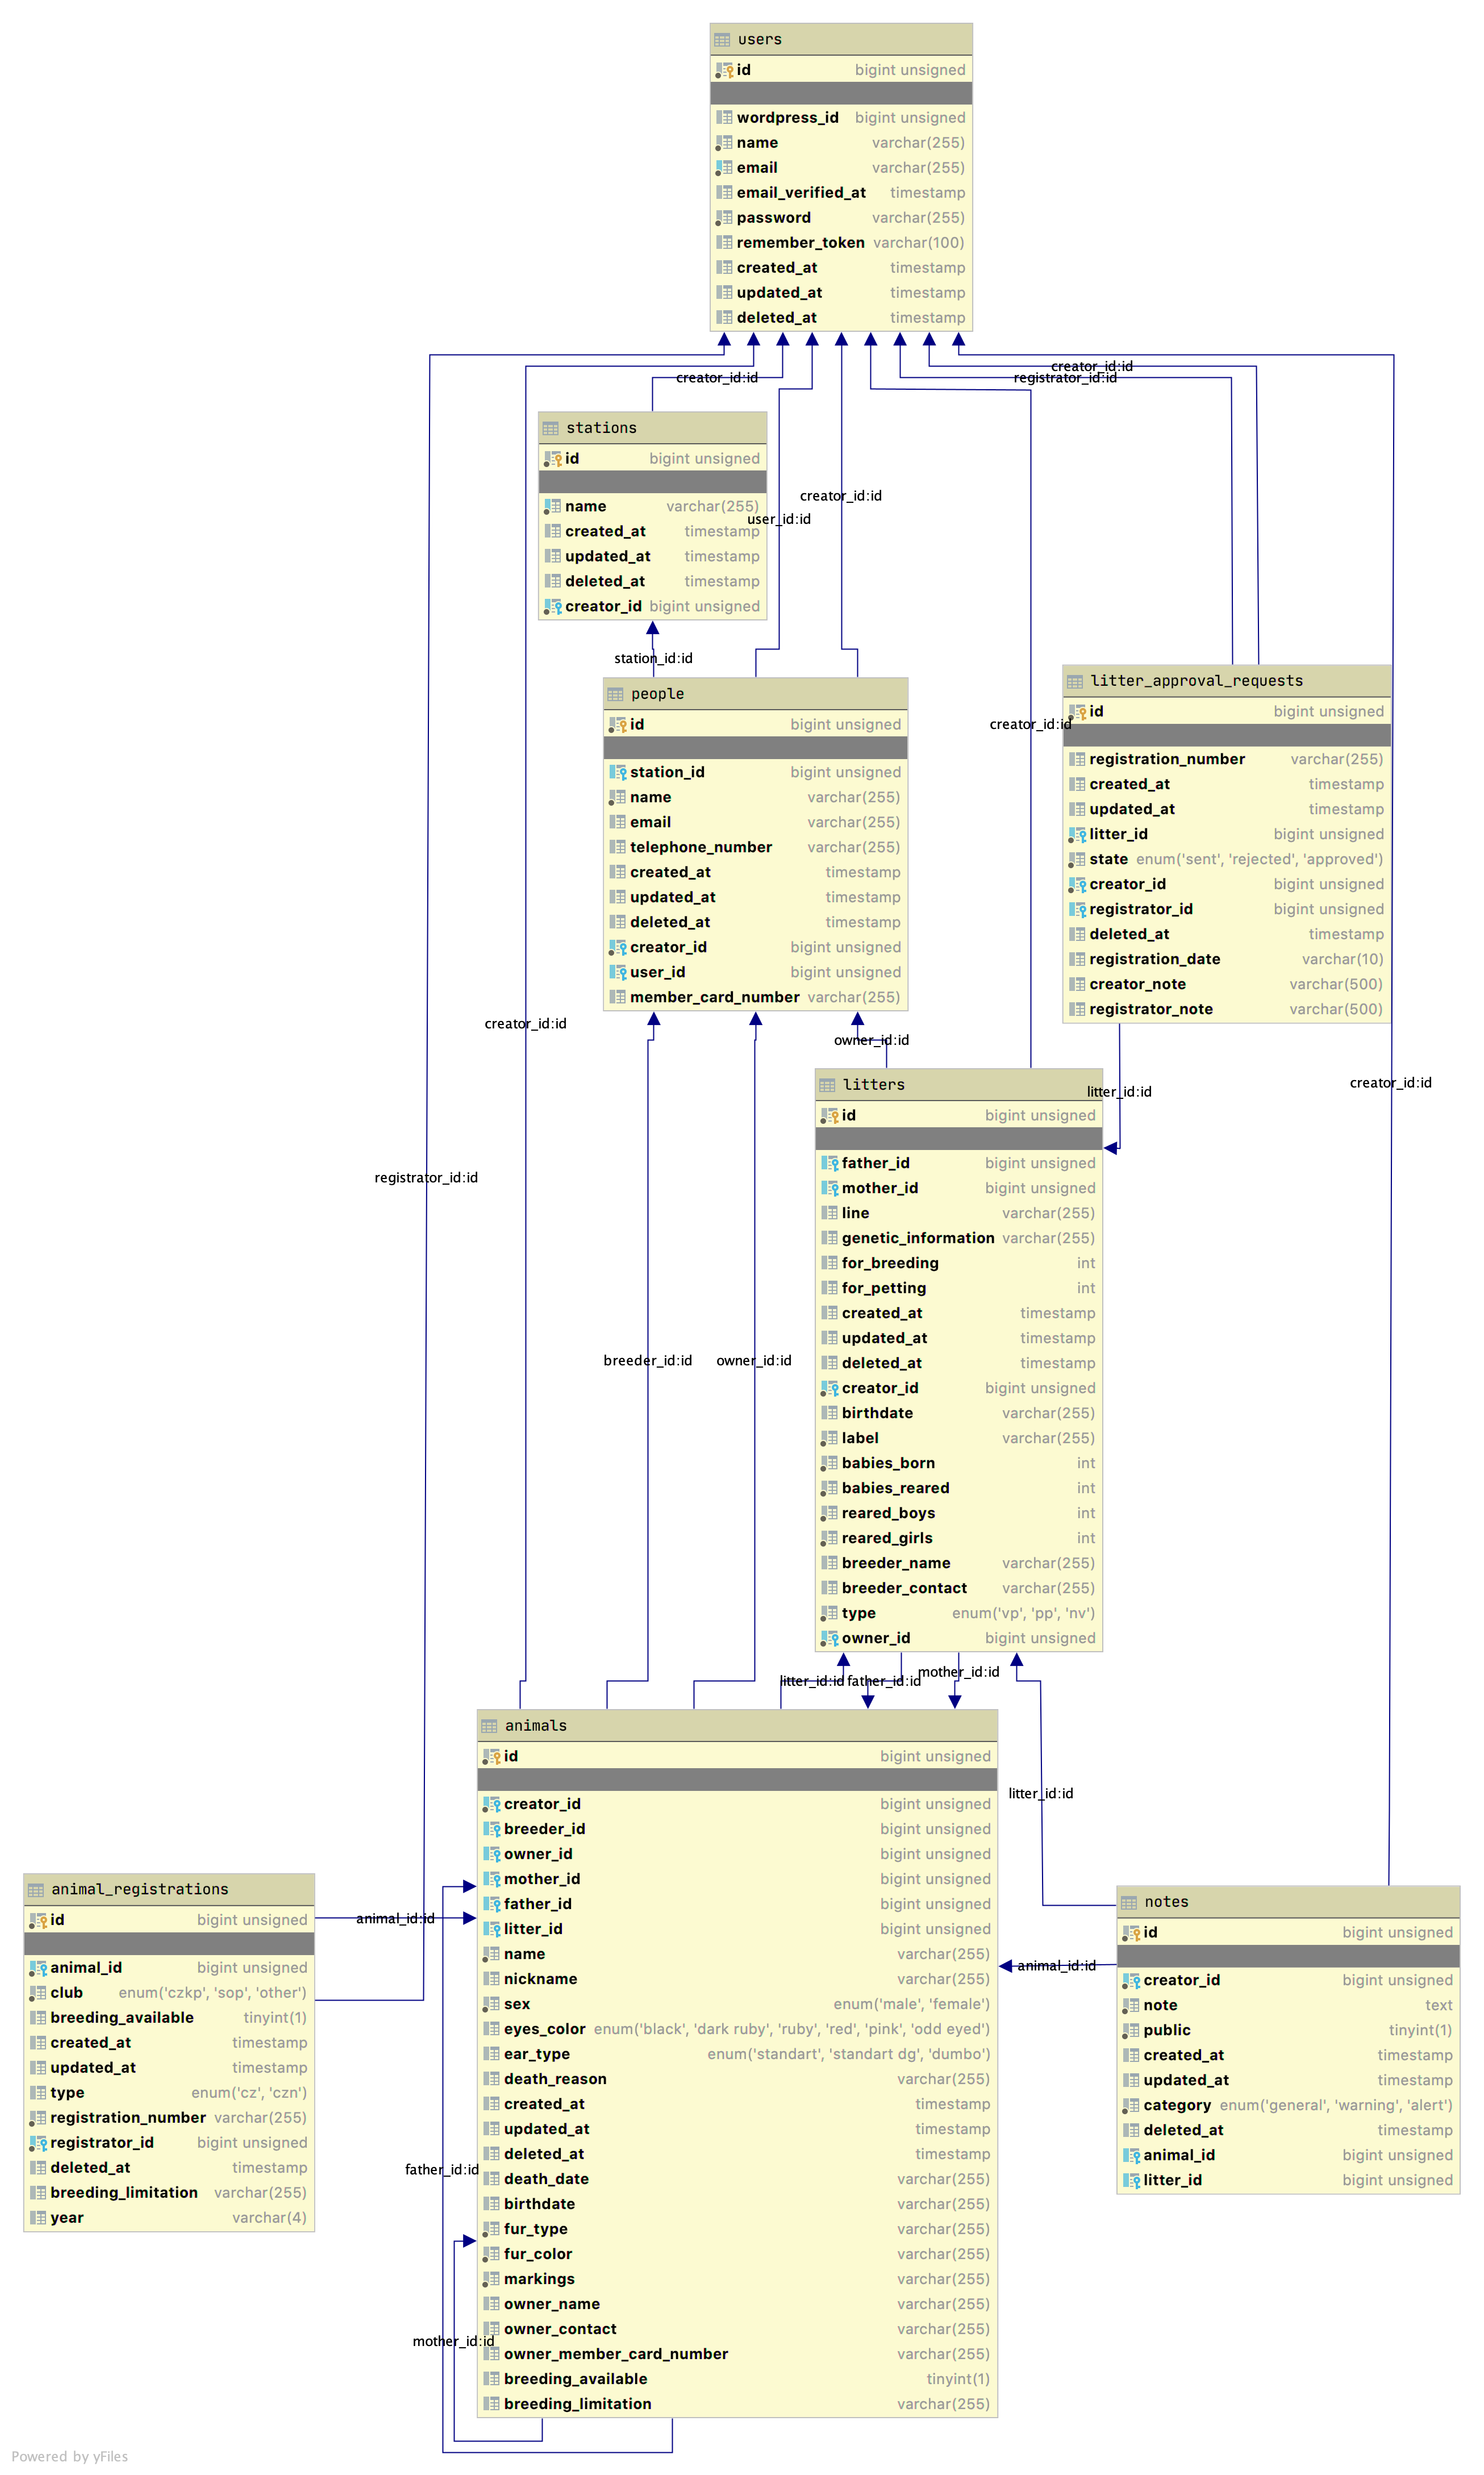
\includegraphics[width=1.0\textwidth]{media/navrh/diagram.png}
	\caption{Logický model databázy}
\end{figure}
